\chapter{Implementacja}
\section{Wprowadzenie}
Celem tego rozdziału jest szczegółowy opis podejścia do realizacji projektu BBS, a mianowicie wyjaśnienie podstawowych pojęć, analiza architektury oraz algorytmów stosowanych do przetwarzania danych.

Chciałbym zacząć od tego, czym właściwie jest BBS. Zgodnie z definicją projekt jest w rzeczywistości procesorem języka \cite{compilers}, a konkretnie tłumaczem według następujących cech, które wynikają bezpośrednio z wymagań opisanych w sekcji 2:
\begin{itemize}
    \item Oprogramowanie analizuje kod wejściowy, napisany w specjalnie opracowanym na potrzeby projektu języku
    \item Oprogramowanie powinno wykrywać i raportować możliwe błędy logiczne lub składniowe w pliku wejściowym
    \item Zamiast tłumaczyć plik wejściowy na inny język programowania, program powinien wykonać polecenia opisane w pliku wejściowym
\end{itemize}

Dodatkowo oprogramowanie to zawiera również preprocesor. Dzieje się tak, aby plik wejściowy mógł zostać podzielony na wiele części, co umożliwi działanie mechanizmu budowania podprojektu.

\section{Struktura interpretera}
Zgodnie ze standardową strukturą kompilatorów i interpreterów, oprogramowanie BBS implementuje część frontend (czyli tę, która przeprowadza analizę) prawie w całości, natomiast backend nie zajmuje się optymalizacją ani generowaniem kodu, ponieważ wykonuje on określone instrukcje na podstawie danych wejściowych (czyli proces syntezy de facto nie zachodzi) \cite{compilers}.

Jeśli patrzyć na dane oprogramowanie ze względu na ogólnie przyjęte fazy kompilacji (które odpowiadają opisanym powyżej częściom standardowego kompilatora lub interpretera), to BBS realizuje prawie wszystkie fazy frontendu, z wyjątkiem generowania kodu pośredniego. Wynika to z niepraktyczności generowania kodu pośredniego bez znaczących opcji jego dalszego wykorzystania. Więc BBS zamiast tej fazy ma swoją, specjalną fazę - fazę wypełniania wewnętrznej struktury opisującej projekt, który ma zostać zbudowany z BBS. Sama konstrukcja, a także procesy zachodzące w tej fazie zostaną szczegółowo opisane w dalszej części.

Podejście do implementacji backendu zasadniczo różni się od standardowego: nie jest wymagane dalsze tłumaczenie kodu na inny język, nie są realizowane fazy generowania kodu w innym języku. Zamiast tego backend na podstawie informacji o projekcie dostarczonych użytkownikowi wybiera określone polecenia do kontrolowania i budowania projektów.

Schemat fazowy BBS wygląda następująco:

\begin{figure}[h]
    \caption{Schemat fazowy projektu BBS}
    \centering
    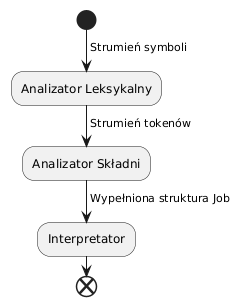
\includegraphics[width=0.4\textwidth]{Images/phases.png}
\end{figure}

Następnie opis procesu implementacji programu zostanie podzielony na części, które również dzielą się na fazy. Ma to na celu proste opisanie procesów zachodzących w środku programu, a także zademonstrowanie danych wejściowych/wyjściowych.

\section{Analiza}
Jak opisano powyżej, dane wejściowe są analizowane w części frontendowej programu. Analizator dzieli dane wejściowe na części i narzuca im strukturę gramatyczną, która później posłuży do zbudowania projektu. Jeżeli parser stwierdzi, że dane wejściowe są niepoprawne składniowo lub semantycznie, informuje o tym użytkownika w najbardziej zrozumiały sposób. Dodatkowo analizator zbiera informacje w postaci tablicy symboli, co zostanie opisane w dalszej części.

\subsection{Analiza leksykalna}
Analiza leksykalna jest pierwszym etapem analizy danych wejściowych. Analizator leksykalny odczytuje strumień symboli i grupuje je w sensowną sekwencję zwaną leksemami, dla których analizator leksykalny generuje tzw. token składający się z typu pary -- odwołanie do tabeli symboli \cite{compilers}.

W projekcie BBS analizator leksykalny jest podzielony na dwie odrębne klasy, \texttt{Lexer} i \texttt{Scanner}, dla których zaimplementowana jest także klasa pomocnicza \texttt{Context}. Także klasy te korzystają z dodatkowych elementów, które zostaną opisane później (ale będą tu omawiane tylko te, które naprawdę zasługują na uwagę, np. nie będzie tu opisu klas wyjątków).

\subsubsection{Klasa Scanner}
Klasa \texttt{Scanner} jest osobną klasą, której delegowana jest rola odczytu plików. To właśnie w tej klasie hermetyzowane są wszelkie operacje sprawdzania istnienia, otwierania i odczytywania plików znak po znaku, a także omijania pustych linii czy komentarzy. Jego implementacja jest dość prosta, gdyż \texttt{Scanner} umożliwia odczytanie bieżącego znaku (funkcja \texttt{Get()}) i przejście do następnego (funkcja \texttt{Move()}). Z kolei operacja \texttt{Get()} opiera się na \texttt{std::optional} \cite{cpp_optional}, innowacji w C++17, która pozwala przechowywać wartość lub nic w bezpieczny i przejrzysty sposób. Klasa na wejściu otrzymuje nazwę pliku do odczytania, a na wyjściu zwraca przeczytany znak (odfiltrowując niepotrzebne), jeśli takie istnieją.

Na szczególną uwagę zasługuje metoda o nazwie \texttt{Skip()} (wywoływana wewnątrz metody \texttt{Move()}), która wykonuje operację pomijania komentarzy i pustych znaków w przypadku konieczności przeczytania kolejnej linii (czyli oznacza, że został znaleziony znak nowej linii). Ta metoda wygląda następująco:

\begin{lstlisting}[label=list:scanner,caption=Metoda Scanner::Skip(),basicstyle=\footnotesize\ttfamily]
void Scanner::Skip()
{
    // Read the next line if scanner finds a new line symbol, a comment or an empty line
    auto character = context_.GetCharacter();
    while(!character || character.value() == constants::kComment)
    {
        std::string line;
        std::getline(file_, line);
        if(file_.fail())
        {
            file_.close();
            return;
        }
    
        context_.Update(std::move(line));
        character = context_.GetCharacter();
    }
    
    // Check if the line still has anything to read
    if(!character || character.value() == '\0')
    {
        file_.close();
    }
}
\end{lstlisting}

Analizując ten kod, możemy stwierdzić, że \texttt{Scanner} najpierw odczytuje bieżący znak, który następnie przechodzi sprawdzenie istnienia (\texttt{std::optional} jest pusty, jeśli znak nie był czytany przez zamknięty plik, np.) lub równość określonego w gramatyce języka symbolu komentarza. Następnie, w przypadku pozytywnego wyniku kontroli (pusty znak lub komentarz), \texttt{Scanner} próbuje odczytać następną linię. Jeśli instrukcja się powiedzie, \texttt{Scanner} aktualizuje kontekst nową linią i zapamiętuje nowy znak jako bieżący, po czym powtarzane jest sprawdzenie istnienia znaku lub komentarza (ponieważ nowa linia może zawierać także komentarz). Przy wyjściu z pętli \texttt{Scanner} sprawdza, czy ostatnia linia została odczytana i jeśli odpowiedź jest pozytywna, plik jest zamykany.

\subsubsection{Klasa Context}
Między innymi moduł \texttt{lexer} zawiera ważną klasę pomocniczą \texttt{Context}, której wpływ na moduł jest dość znaczący. Klasa ta pojawiła się w procesie rozbudowy i rozwoju projektu BBS poprzez wyodrębnienie metod i pól z klasy \texttt{Scanner} w celu nie tylko spełnienia zasad SOLID \cite{solid}, ale także ułatwienia dostępu do informacji o bieżącej lokalizacji w pliku. Funkcjonalność ta służy w szczególności szczegółowemu informowaniu użytkownika o błędach składniowych lub semantycznych.

Klasa \texttt{Context} zawiera bieżącą linię przetwarzaną przez program, jej indeks w pliku oraz pozycję bieżącego znaku w linii. Wszystkie pola są chronione i dostępne pośrednio poprzez predefiniowany interfejs.

\subsubsection{Klasa Lexer}
Klasa \texttt{Lexer}, jak sama nazwa wskazuje, jest implementacją analizatora leksykalnego. Ta klasa jest najbardziej złożona ze wszystkich w module, a jej struktura jest modułowa, co ułatwia zmianę jej elementów w miarę zmiany wymagań lub gramatyki języka.

Główna klasa \texttt{Lexer} ma tylko metody manipulacji tokenami (\texttt{Get()} do odczytania bieżącego tokena i \texttt{Next()} do żądania odczytania następnego tokena), ponieważ praca z plikami została delegowany do klasy \texttt{Scanner}.

Proces kategoryzacji tokenów został delegowany do szeregu klas zwanych procedurami obsługi. Klasy te stanowią implementację wzorca projektowego „Łańcuch odpowiedzialności” \cite{cor}, który polega na przetwarzaniu określonych żądań przez dany obiekt i ich późniejszym przekazywaniu do kolejnych obiektów, w przypadku gdyby żądanie nie powiodło się. Ten wzorzec został użyty, aby wycofać użycie \texttt{switch-case}, aby umożliwić znacznie łatwiejsze (i jednolite) podłączanie nowych klas obsługi przy minimalnych zmianach w istniejącym kodzie (zgodnie z zasadami SOLID \cite{solid}). Klasy te posiadają następujący interfejs:

\begin{lstlisting}[label=list:handler,caption=Klasa Handler,basicstyle=\footnotesize\ttfamily]
/**
 * @brief A default Lexer input handler, an implementation of the CoR pattern
 * 
 */
class Handler
{
    using Token = parser::tokens::Token;
    
public:
    /**
     * @brief Process the input and return the token if possible
     * 
     * @param scanner - the source of characters to process
     * @return std::unique_ptr<Token> - a pointer to the token or nullptr 
     */
    virtual std::unique_ptr<Token> Process(Scanner& scanner) const;
    
    /**
     * @brief Set the next handler to be called to process the input
     * 
     * @param next - a pointer to the next handler to be called
     */
    void SetNext(std::unique_ptr<Handler> next);
    
protected:
    /**
     * @brief A pointer to the handler, next on the line to process the input
     * 
     */
    std::unique_ptr<Handler> next_;
};
\end{lstlisting}

Oznacza to, że każdy obiekt przetwarzający po utworzeniu otrzymuje łącze do następcy, do którego zostanie przekazane żądanie w przypadku niepowodzenia podczas jego realizacji. Jeśli żaden z programów obsługi nie był w stanie przetworzyć żądania, ostatni w łańcuchu tworzy wyjątek. Implementacja ta pozwoliła maksymalnie uprościć klasę \texttt{Lexer}, kod metody \texttt{Next()}, która wymusza na parserze odczytanie kolejnego tokena z pliku, dzięki wzorcowi "łańcuch odpowiedzialności" \cite{cor} został uproszczony do następującej postaci bez poświęcania stabilności i bezpieczeństwa programu:

\begin{lstlisting}[label=list:scanner,caption=Metoda Lexer::Next(),basicstyle=\footnotesize\ttfamily]
std::shared_ptr<Lexer::Token> Lexer::Next()
{
    token_ = std::move(handler_->Process(scanner_));
    return token_;
}
\end{lstlisting}

Klasa \texttt{Lexer} na wejściu otrzymuje nazwę pliku (która jest przekazywana do obiektu klasy Scanner i nie jest zapisywana bezpośrednio), na wyjściu \texttt{Lexer} zwraca aktualny token, a także umożliwia odczytanie nowy. W przypadku znalezienia nieznanych symboli, których nie przewidywała gramatyka języka, analizator tworzy odpowiedni wyjątek ze szczegółowym opisem położenia symbolu i przyczyną błędu.

Lista tokenów, które program może przetworzyć, odpowiada podanemu językowi i została opisana w sekcji ''Gramatyk języka''.